%
%
%
%

\section{Results}
\label{sec:results}
To demonstrate the functionality of zigzag persistence for analyzing temporal graphs, we will use two examples. 
The first is an analysis of transportation data from Great Britain in Section~\ref{ssec:GB_results}. 
The second is a simulated dataset from the Lorenz system that exhibits intermittency, a dynamical system phenomenon where the dynamic state transition from periodic to chaotic in irregular intervals with results in Section~\ref{ssec:TOPN_results}. 
We study this signal using the temporal ordinal partition network framework as described in Section~\ref{ssec:temp_OPN}.
We compare our results for both examples to some standard networks tools to analyze temporal networks. Namely, we will compare two connectivity statistics and three centrality statistics. 

The two connectivity statistics analyze the Connected Components (CCs). The first CC statistic is the number of connected components $N_{cc}$, which provides a simple shape summary of the graph snapshots by understanding the number of disconnected subgraphs. The second statistic is the average size (number of nodes) of the connected components $\bar{S}_{cc}$. This statistic provides insight into how significant the components are for each graph snapshot.

The second statistic type is on centrality measures. The three centrality measures we use are the average and standardized degree centrality $\bar{C}_d$, betweenness centrality $\bar{C}_b$, and closeness centrality $\bar{C}_c$. 
The degree centrality measures the number of edges connected to a node, the betweenness centrality measures how often a node is used in all possible shortest paths, and the closeness centrality measures how close the node is to all other nodes through the shortest path.
For details on the implementation of each centrality measure, we direct the reader to~\cite{Landherr2010}.




\subsection{Great Britain Temporal Transportation Network} \label{ssec:GB_results}

\begin{figure}%
     \centering
     %
     \begin{minipage}{0.31\textwidth}
         \centering
         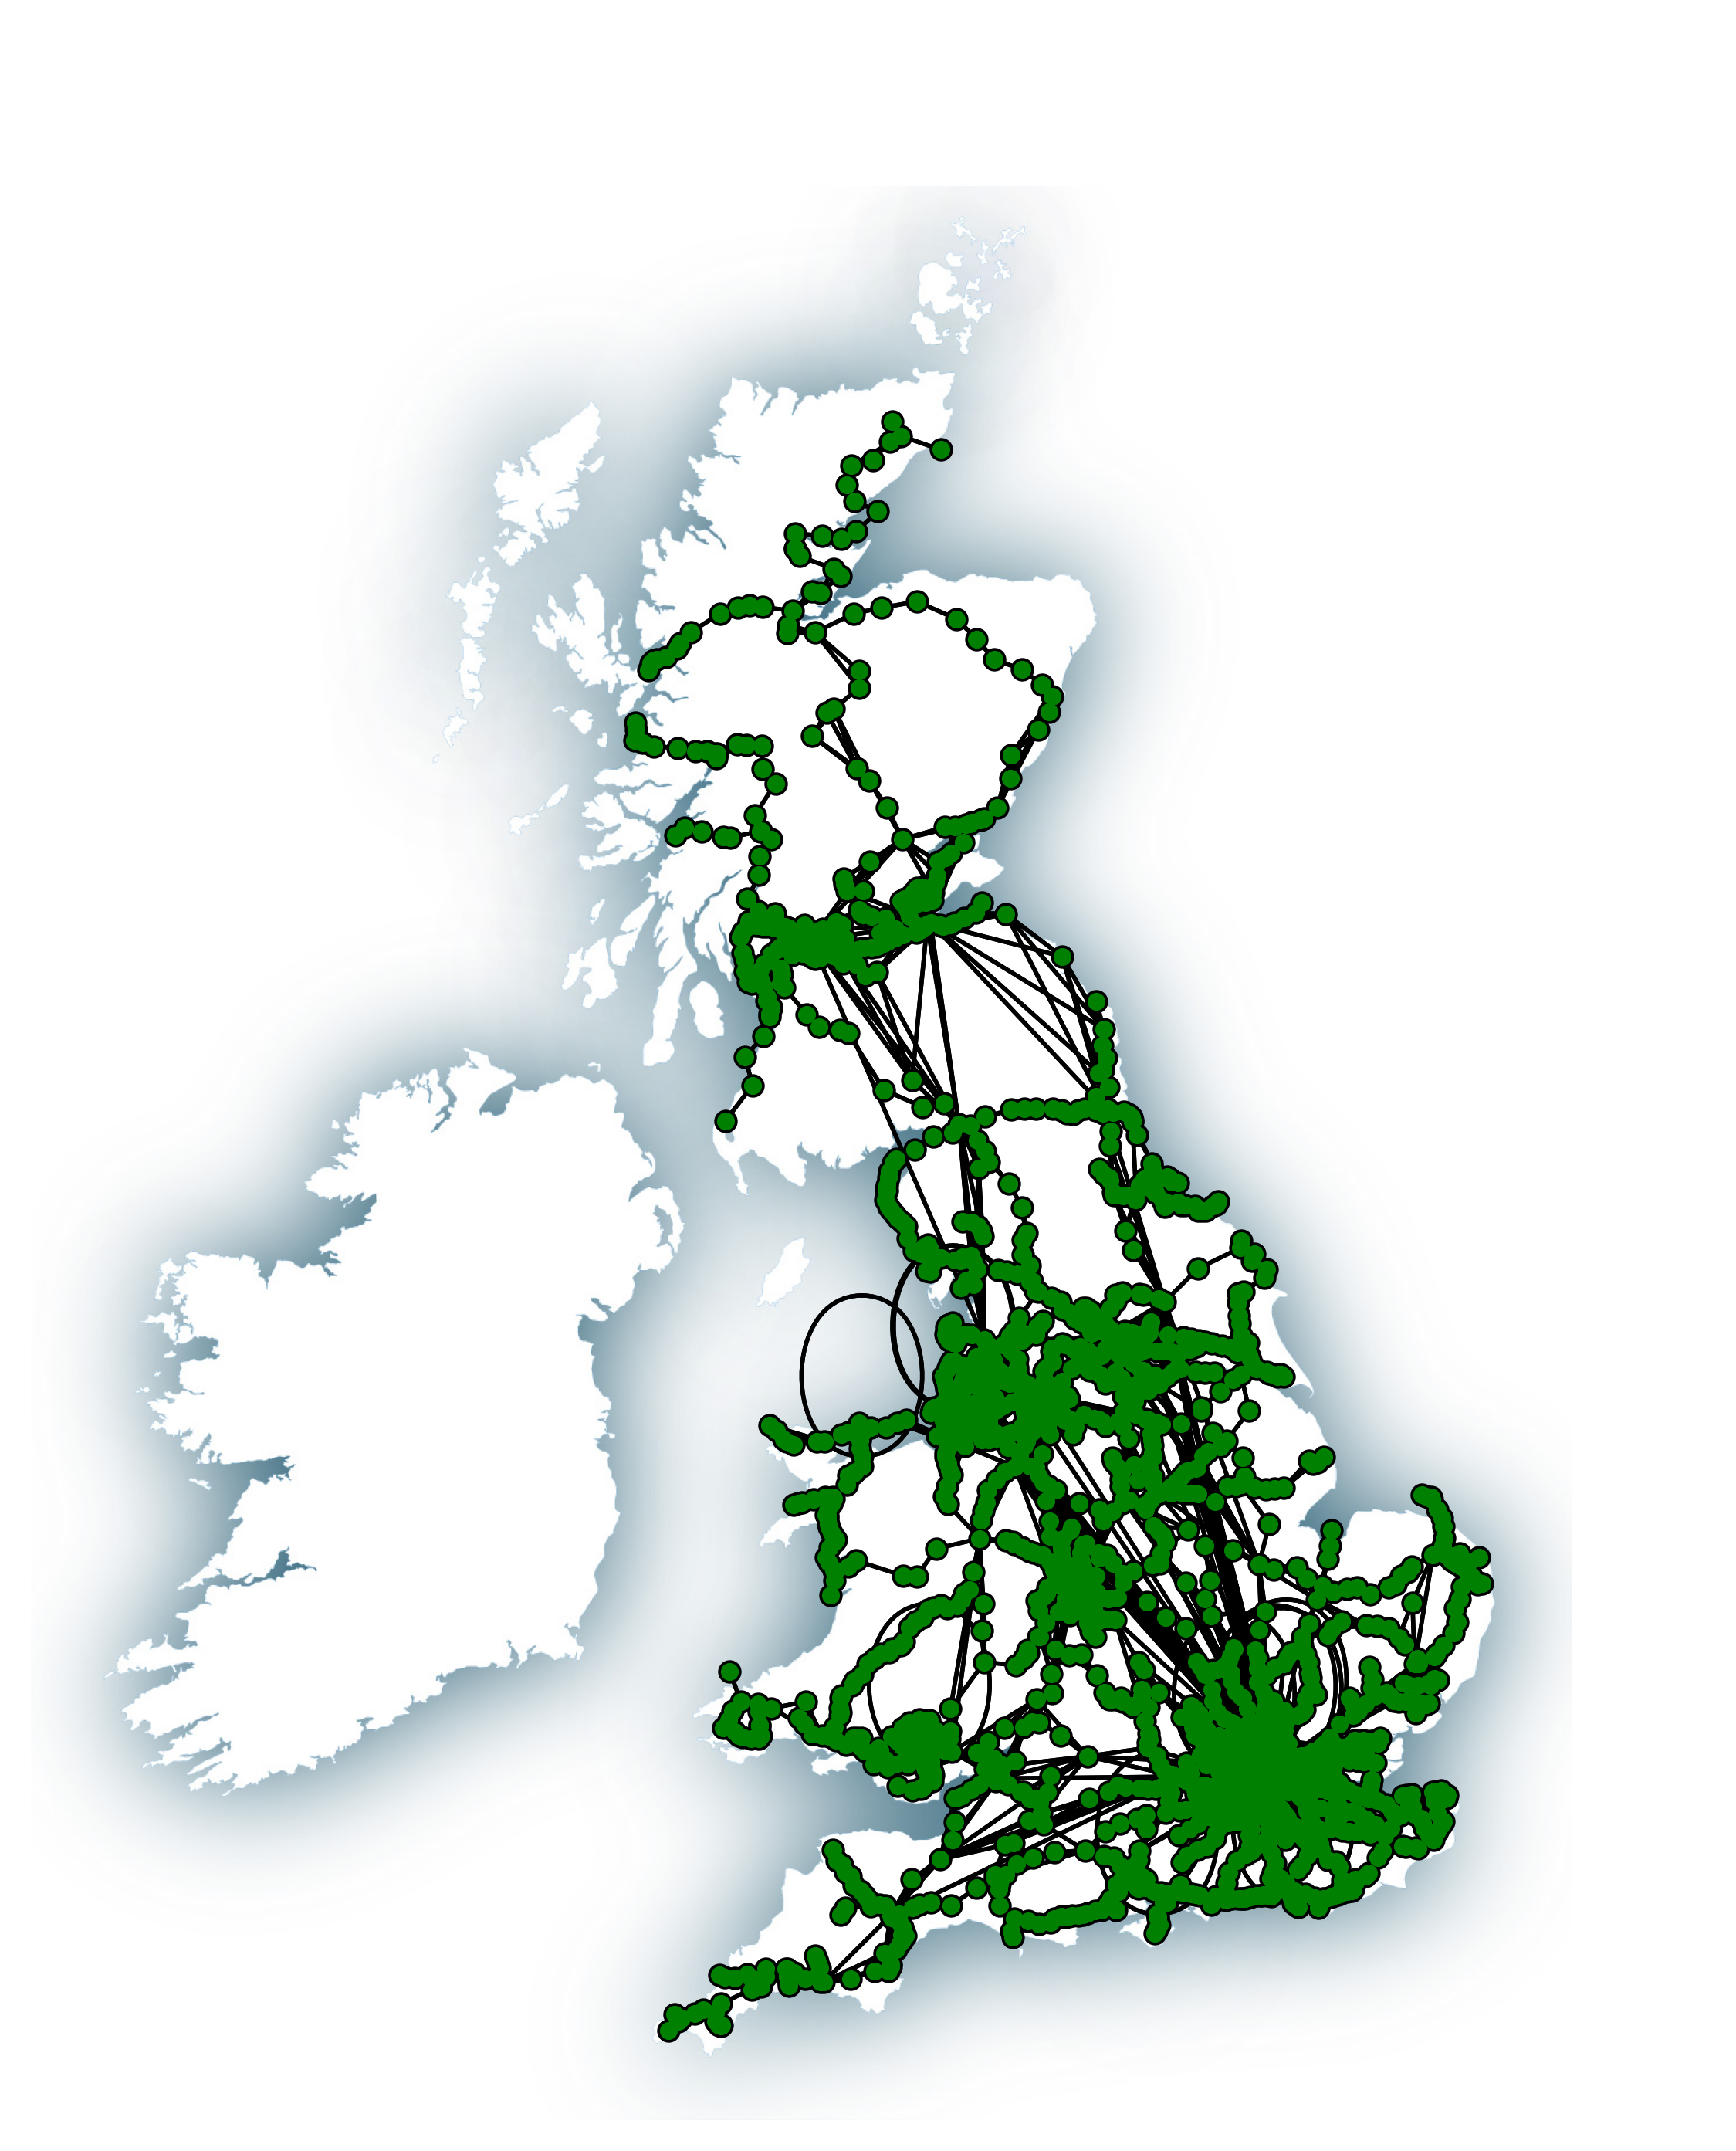
\includegraphics[width=\textwidth]{Figures/GB_rail} 
     \end{minipage}
     \hfill
     \begin{minipage}{0.31\textwidth}
         \centering
         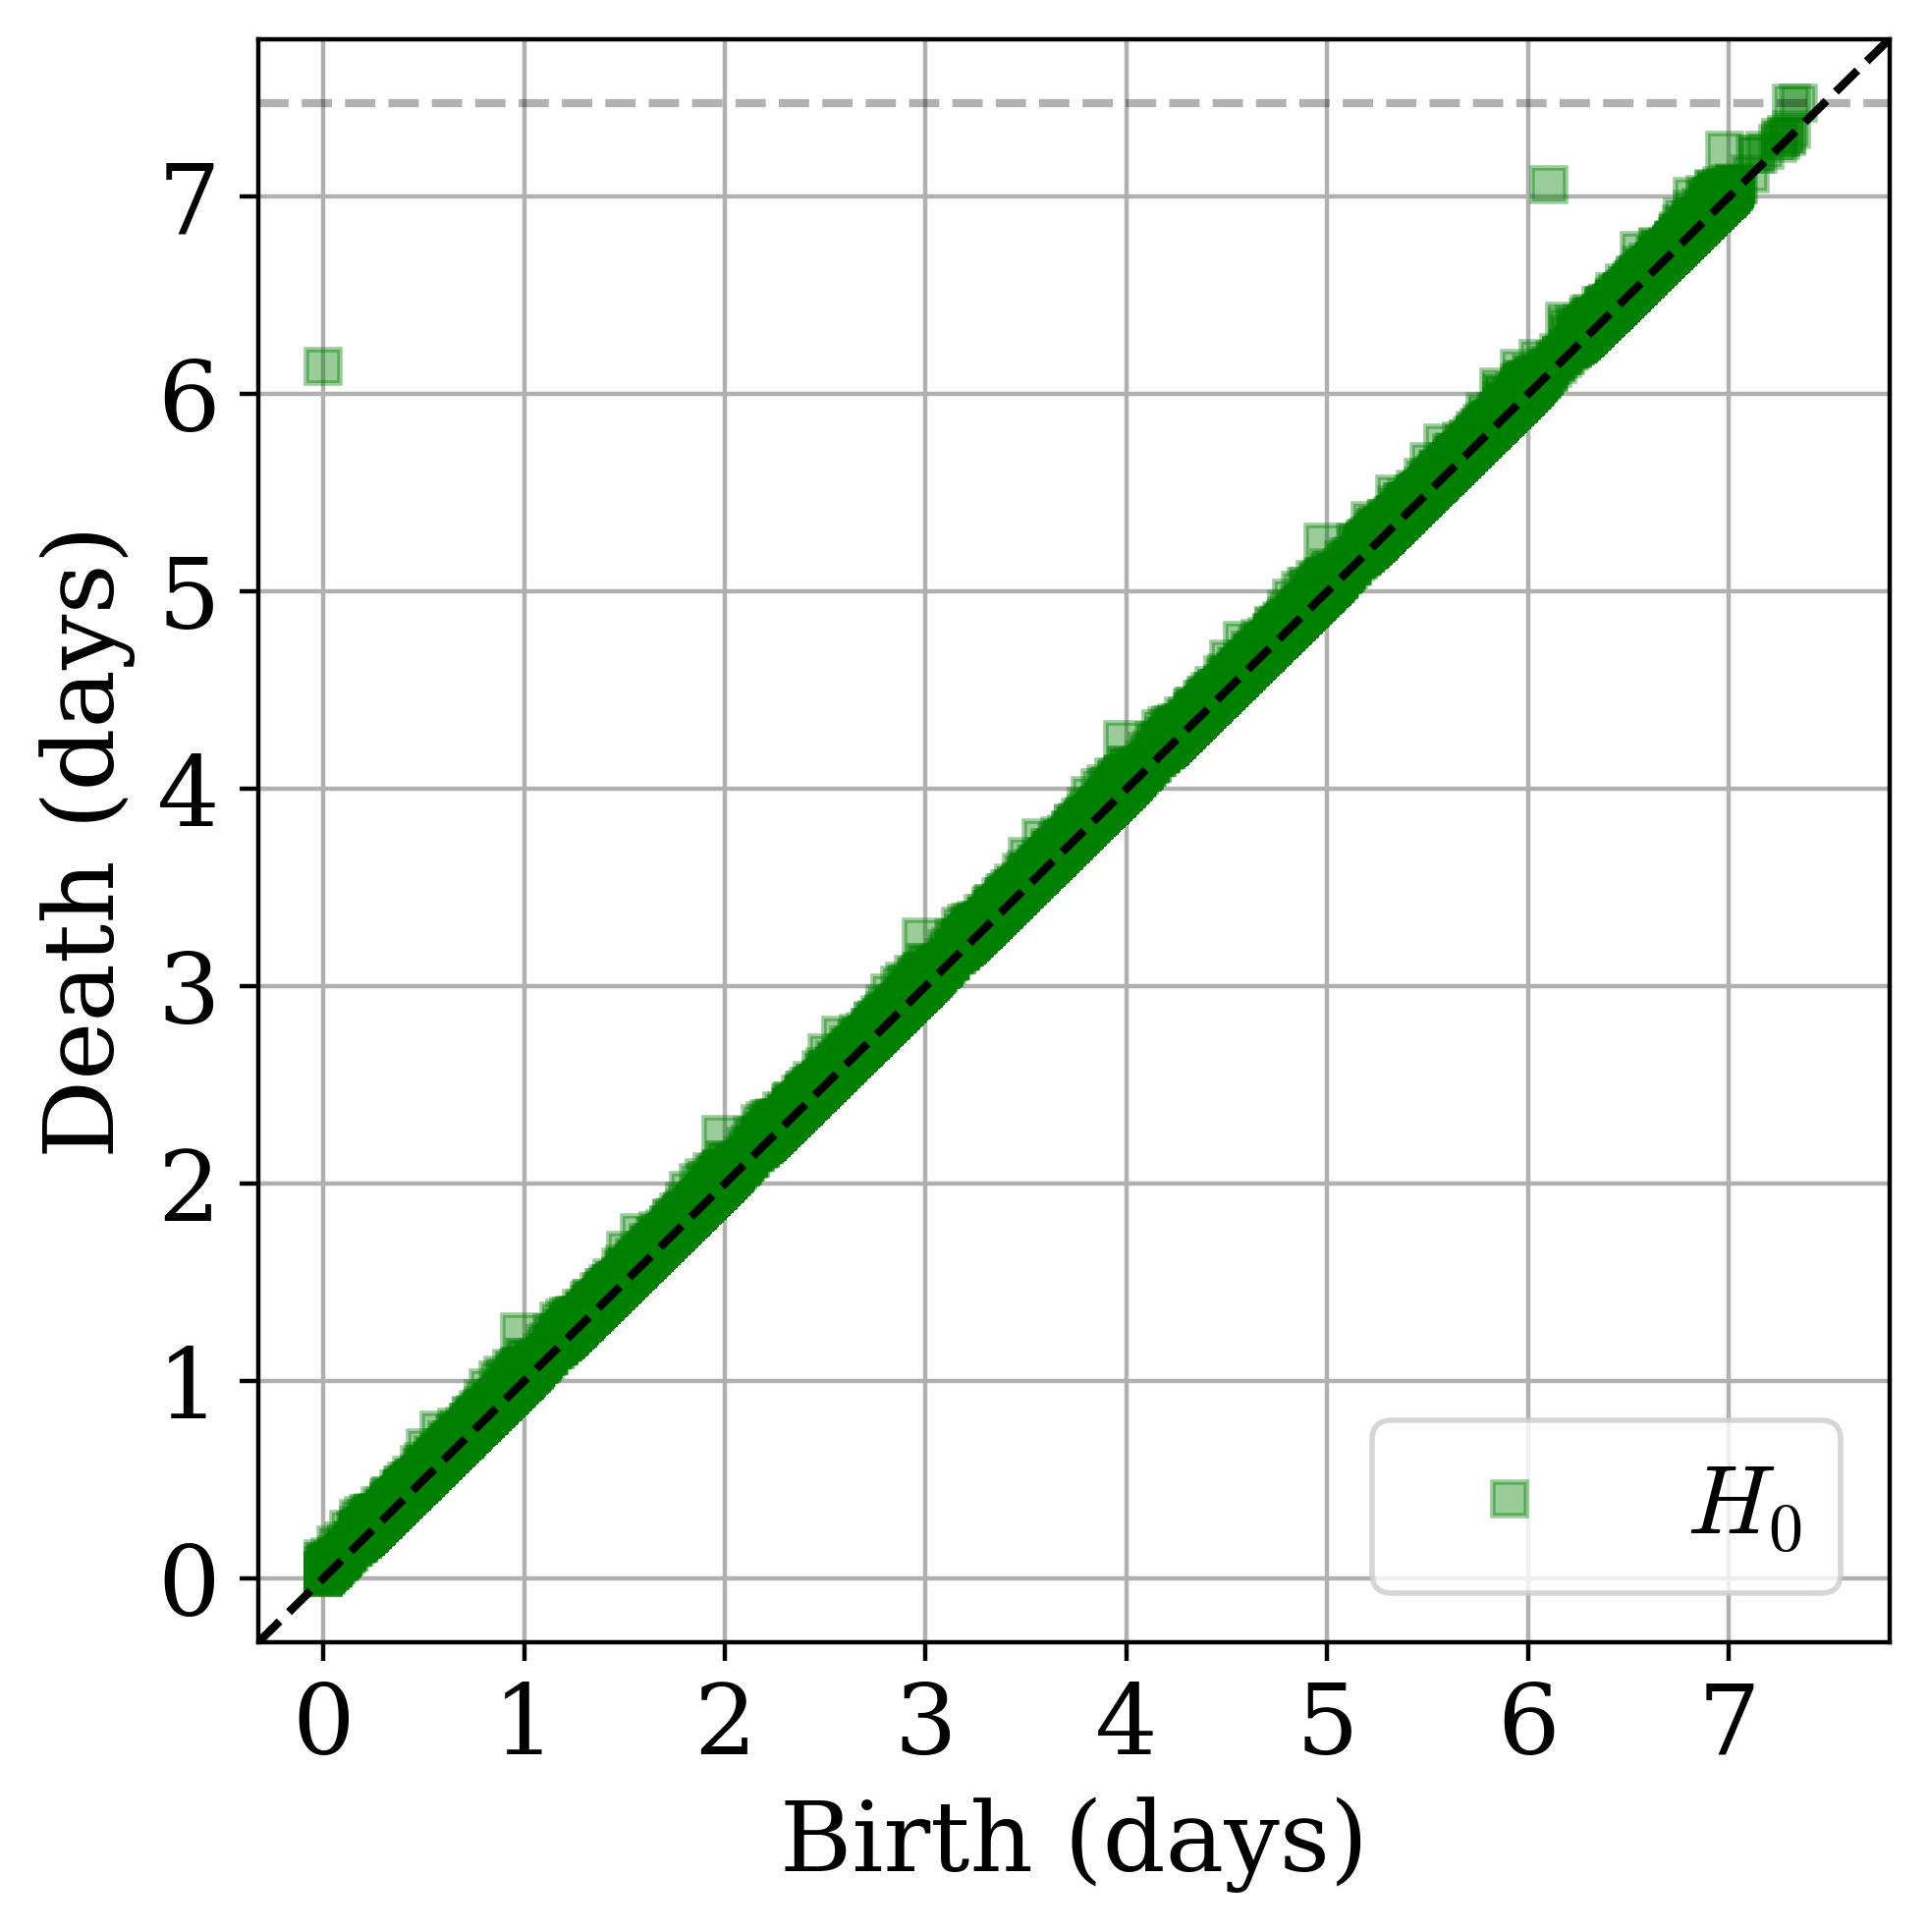
\includegraphics[width=\textwidth]{Figures/GB_rail_PD0_Rips1} 
     \end{minipage}
     \hfill
     \begin{minipage}{0.31\textwidth}
         \centering
         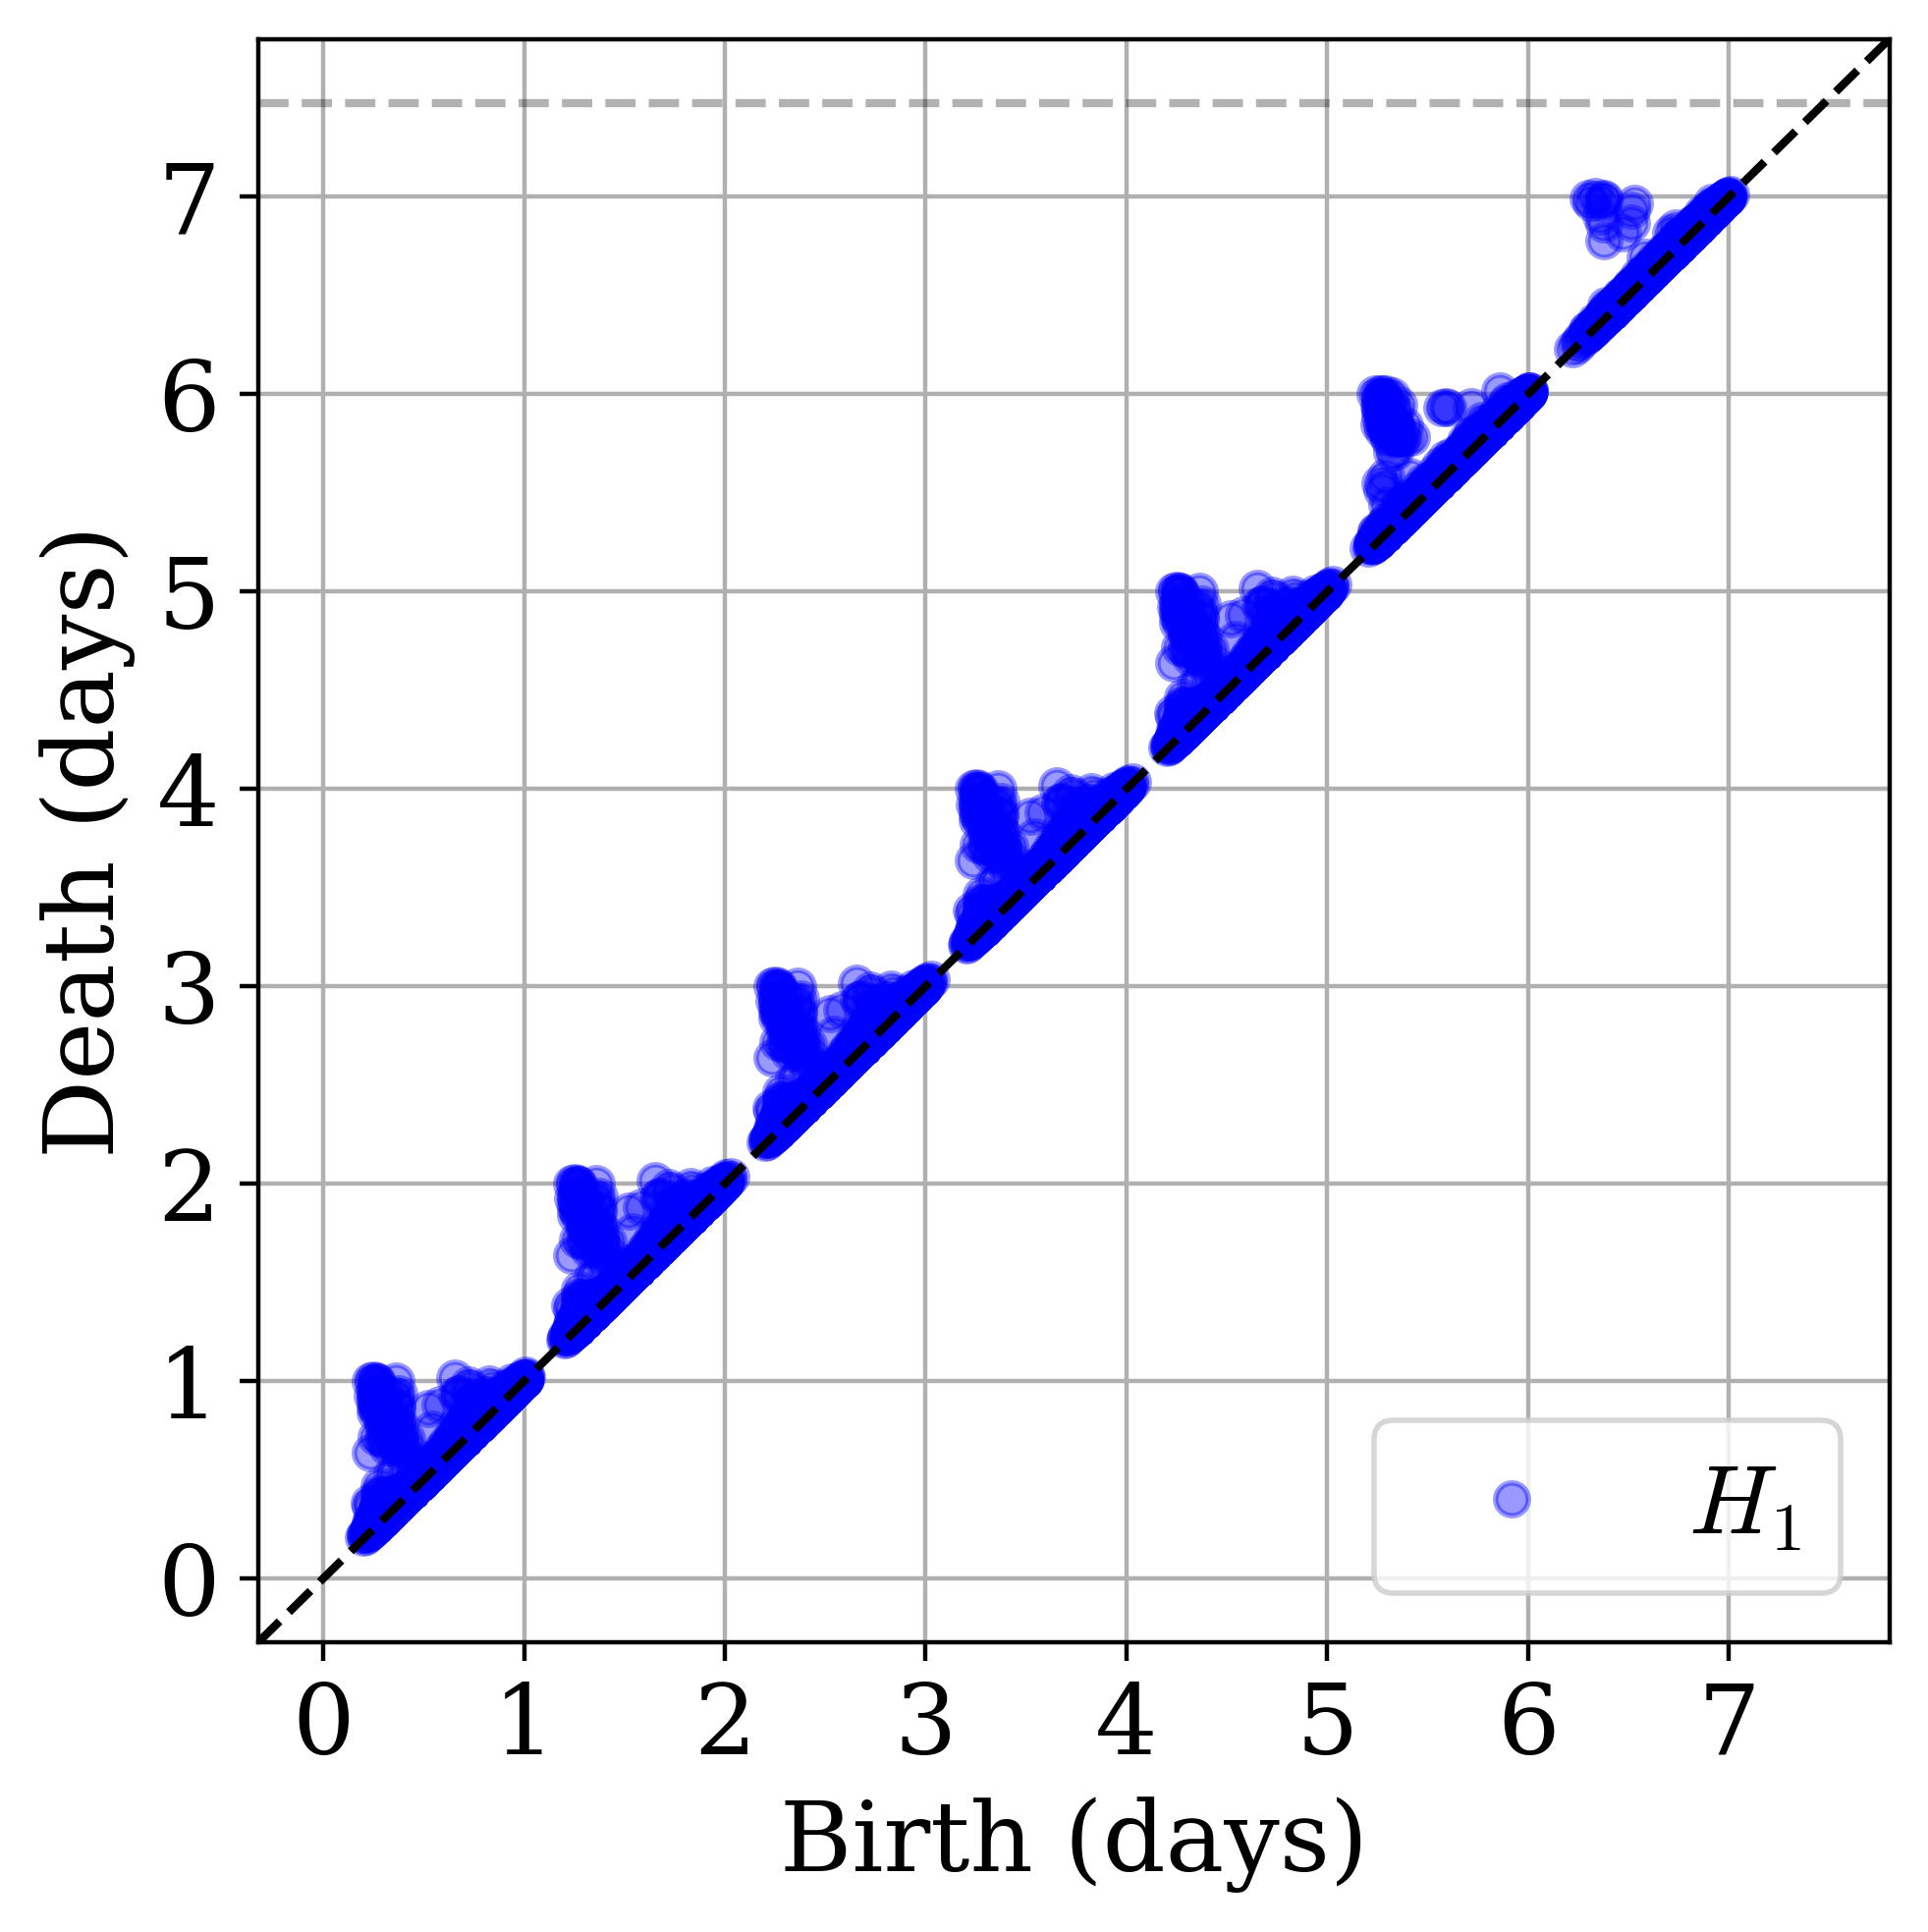
\includegraphics[width=\textwidth]{Figures/GB_rail_PD1_Rips1}
         %
     \end{minipage}

     \begin{minipage}{0.31\textwidth}
         \centering
         (a) Full Rail Travel Network.    
     \end{minipage}
     \hfill
     \begin{minipage}{0.31\textwidth}
         \centering
         (b) Zero-dimensional zigzag persistence.
     \end{minipage}
     \hfill
     \begin{minipage}{0.31\textwidth}
         \centering
         (c) One-dimensional zigzag persistence.
     \end{minipage}
     %
     \caption{Zigzag persistence diagrams of the rail transportation network of Great Britain.}
     \label{fig:GB_rail_network_and_PDs}
\end{figure}
We use temporal networks created from the Great Britain (GB) temporal transportation dataset~\cite{Gallotti2015} for the air, rail, and coach transportation methods.
This data provides the destinations (nodes) and connections (edges) for public transportation in GB. 
Additionally, the departure and arrival times are provided to allow a temporal analysis. This temporal data was collected for one week, Monday through Sunday.
In this section, we use both the rail and coach data; similar calculations for air data are included in Appendix \ref{app:air_and_coach}.
The rail graph constructed without the inclusion of temporal information is shown at left in Fig.~\ref{fig:GB_rail_network_and_PDs} where the destinations are overlaid with a GB map outline. 
Figures for the similar air and coach graphs are included in Appendix \ref{app:air_and_coach}. 
In all three cases, we set the sliding windows to have width $w = 20$ minutes. 
Because the average wait time was 7 minutes and 7 seconds with a standard deviation of 7 minutes and 24 seconds from a collected sample~\cite{vanHagen2011}, this ensures that we retain connectivity. 
Additionally, we used an overlap of 50\% between adjacent windows.%






\subsubsection{Rail}
\begin{figure}
    \centering
    
\includegraphics[width=0.99\textwidth]{GB_rail_mean_centrality_components_analysis}
    \caption{Connectivity and centrality analysis on temporal Great Britain rail network.}
    \label{fig:GB_rail_mean_centrality_components_analysis}
\end{figure}
We first focus on the rail data, for which we use the VR complex with $r=1$.
The 0- and 1-dimensional zigzag diagrams are shown in Fig.~\ref{fig:GB_rail_network_and_PDs}. 
The first noticeable feature is that the 1-dimensional diagram has a clear daily pattern of points, implying that there are many loops in the rail network that persist during the day, but become disconnected in the evenings when the trains are no longer running. 
However, there is still an overarching connectivity of the rail network seen during the week, as noted by the high persistence point at approximately $(0,6)$ in the 0-dimensional diagram. 
We note that this does not mean that the entire graph is connected for the entirety of the days Monday through Saturday, but instead that there is some connected area that remains running even overnight.
We suspect this would be tied to some of the more urban areas such as London, but further work would be needed to implement code to obtain generators of the zigzag diagram. 
This lower connectivity on Saturday and Sunday can also be seen in the additional sparsity in the day 6 and day 7 peaks in the 1-dimensional diagram. 

We compare these interpretations to the standard graph analysis tools \cite{Holme2015}. 
The standard centrality and connectivity statistics for the same data are shown in Fig.~\ref{fig:GB_rail_mean_centrality_components_analysis}.
We can clearly see that there is a daily periodicity in the data from these standard tools as was seen in the zigzag persistence. 
Specifically, all the connectivity and centrality measures increase during peak travel hours. 
What is lost, and which can be augmented with the zigzag viewpoint, is the ability to connect the clustering and centrality measures from one time step to the next. 
There is no way to determine, say, from the $N_{cc}$ graph that there is some portion of the graph that remains connected for 6 out of the 7 days. 
For this reason, we believe that the zigzag setting can be used along side the standard measures in order to strengthen analysis of given temporal graph information. 





%



\begin{figure}%
     \centering
     %
     \begin{minipage}{0.31\textwidth}
         \centering
         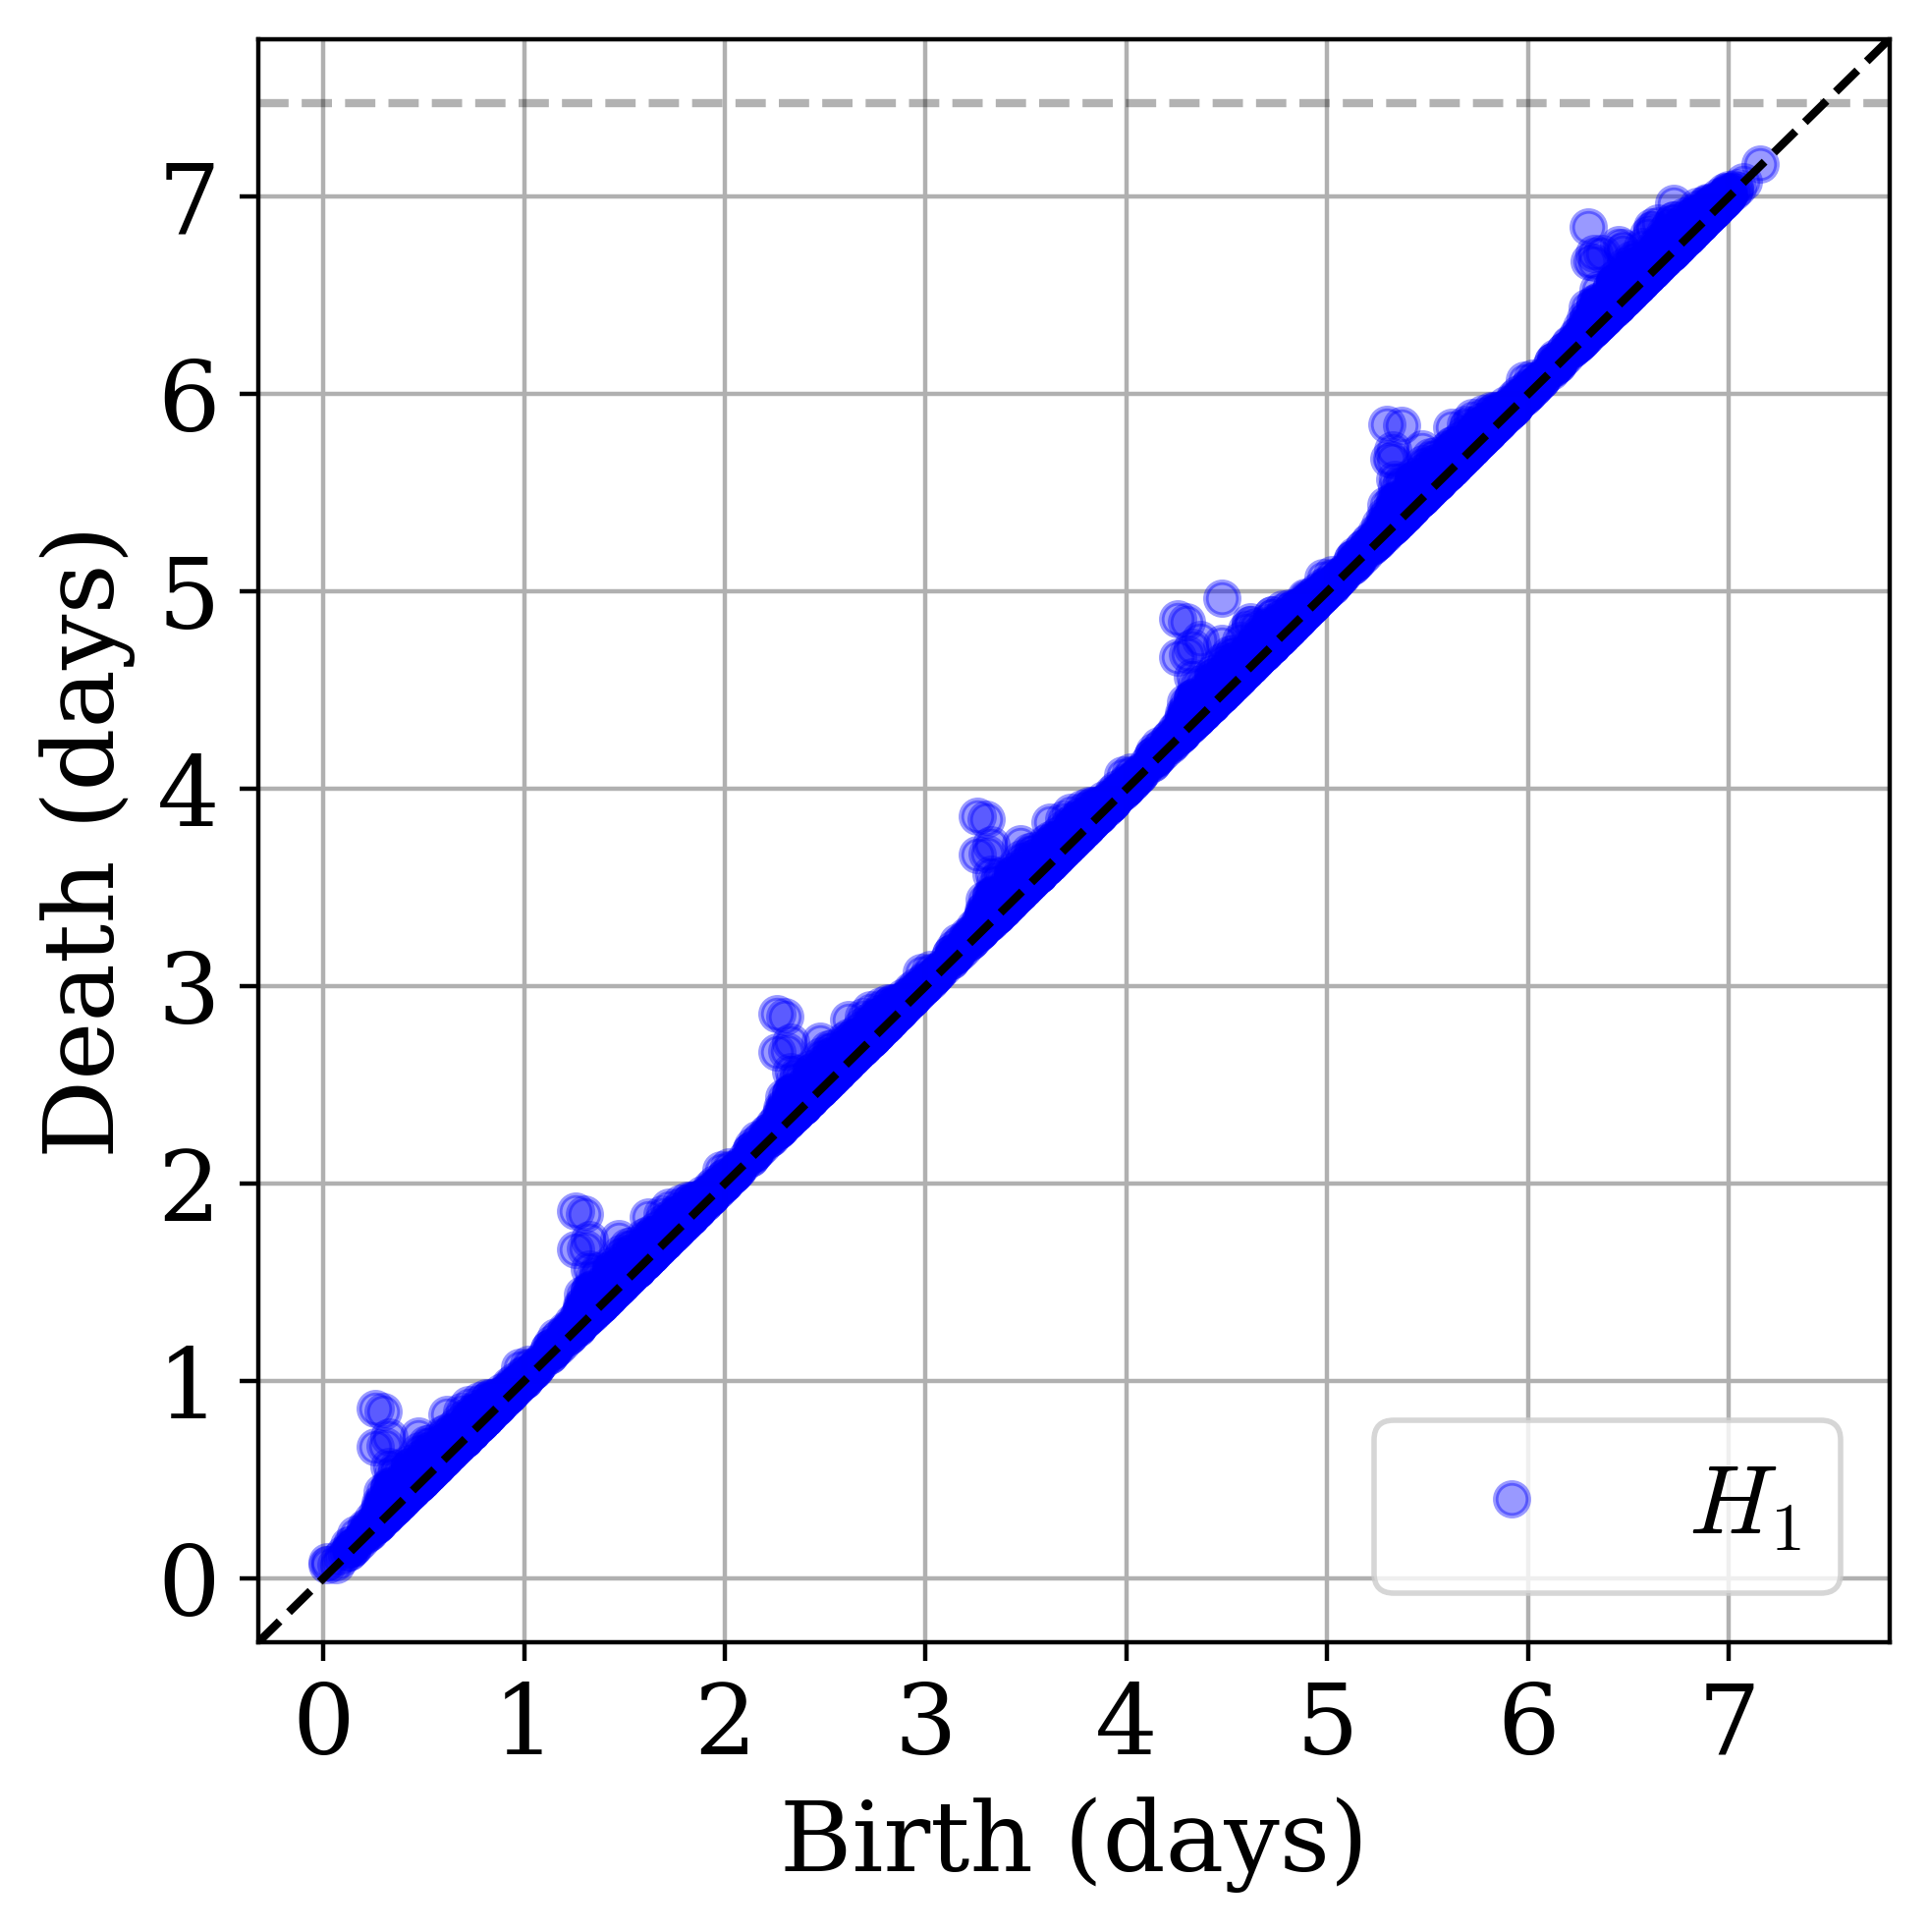
\includegraphics[width=\textwidth]{Figures/GB_coach_PD1}
     \end{minipage}
     \hfill
     \begin{minipage}{0.31\textwidth}
         \centering
         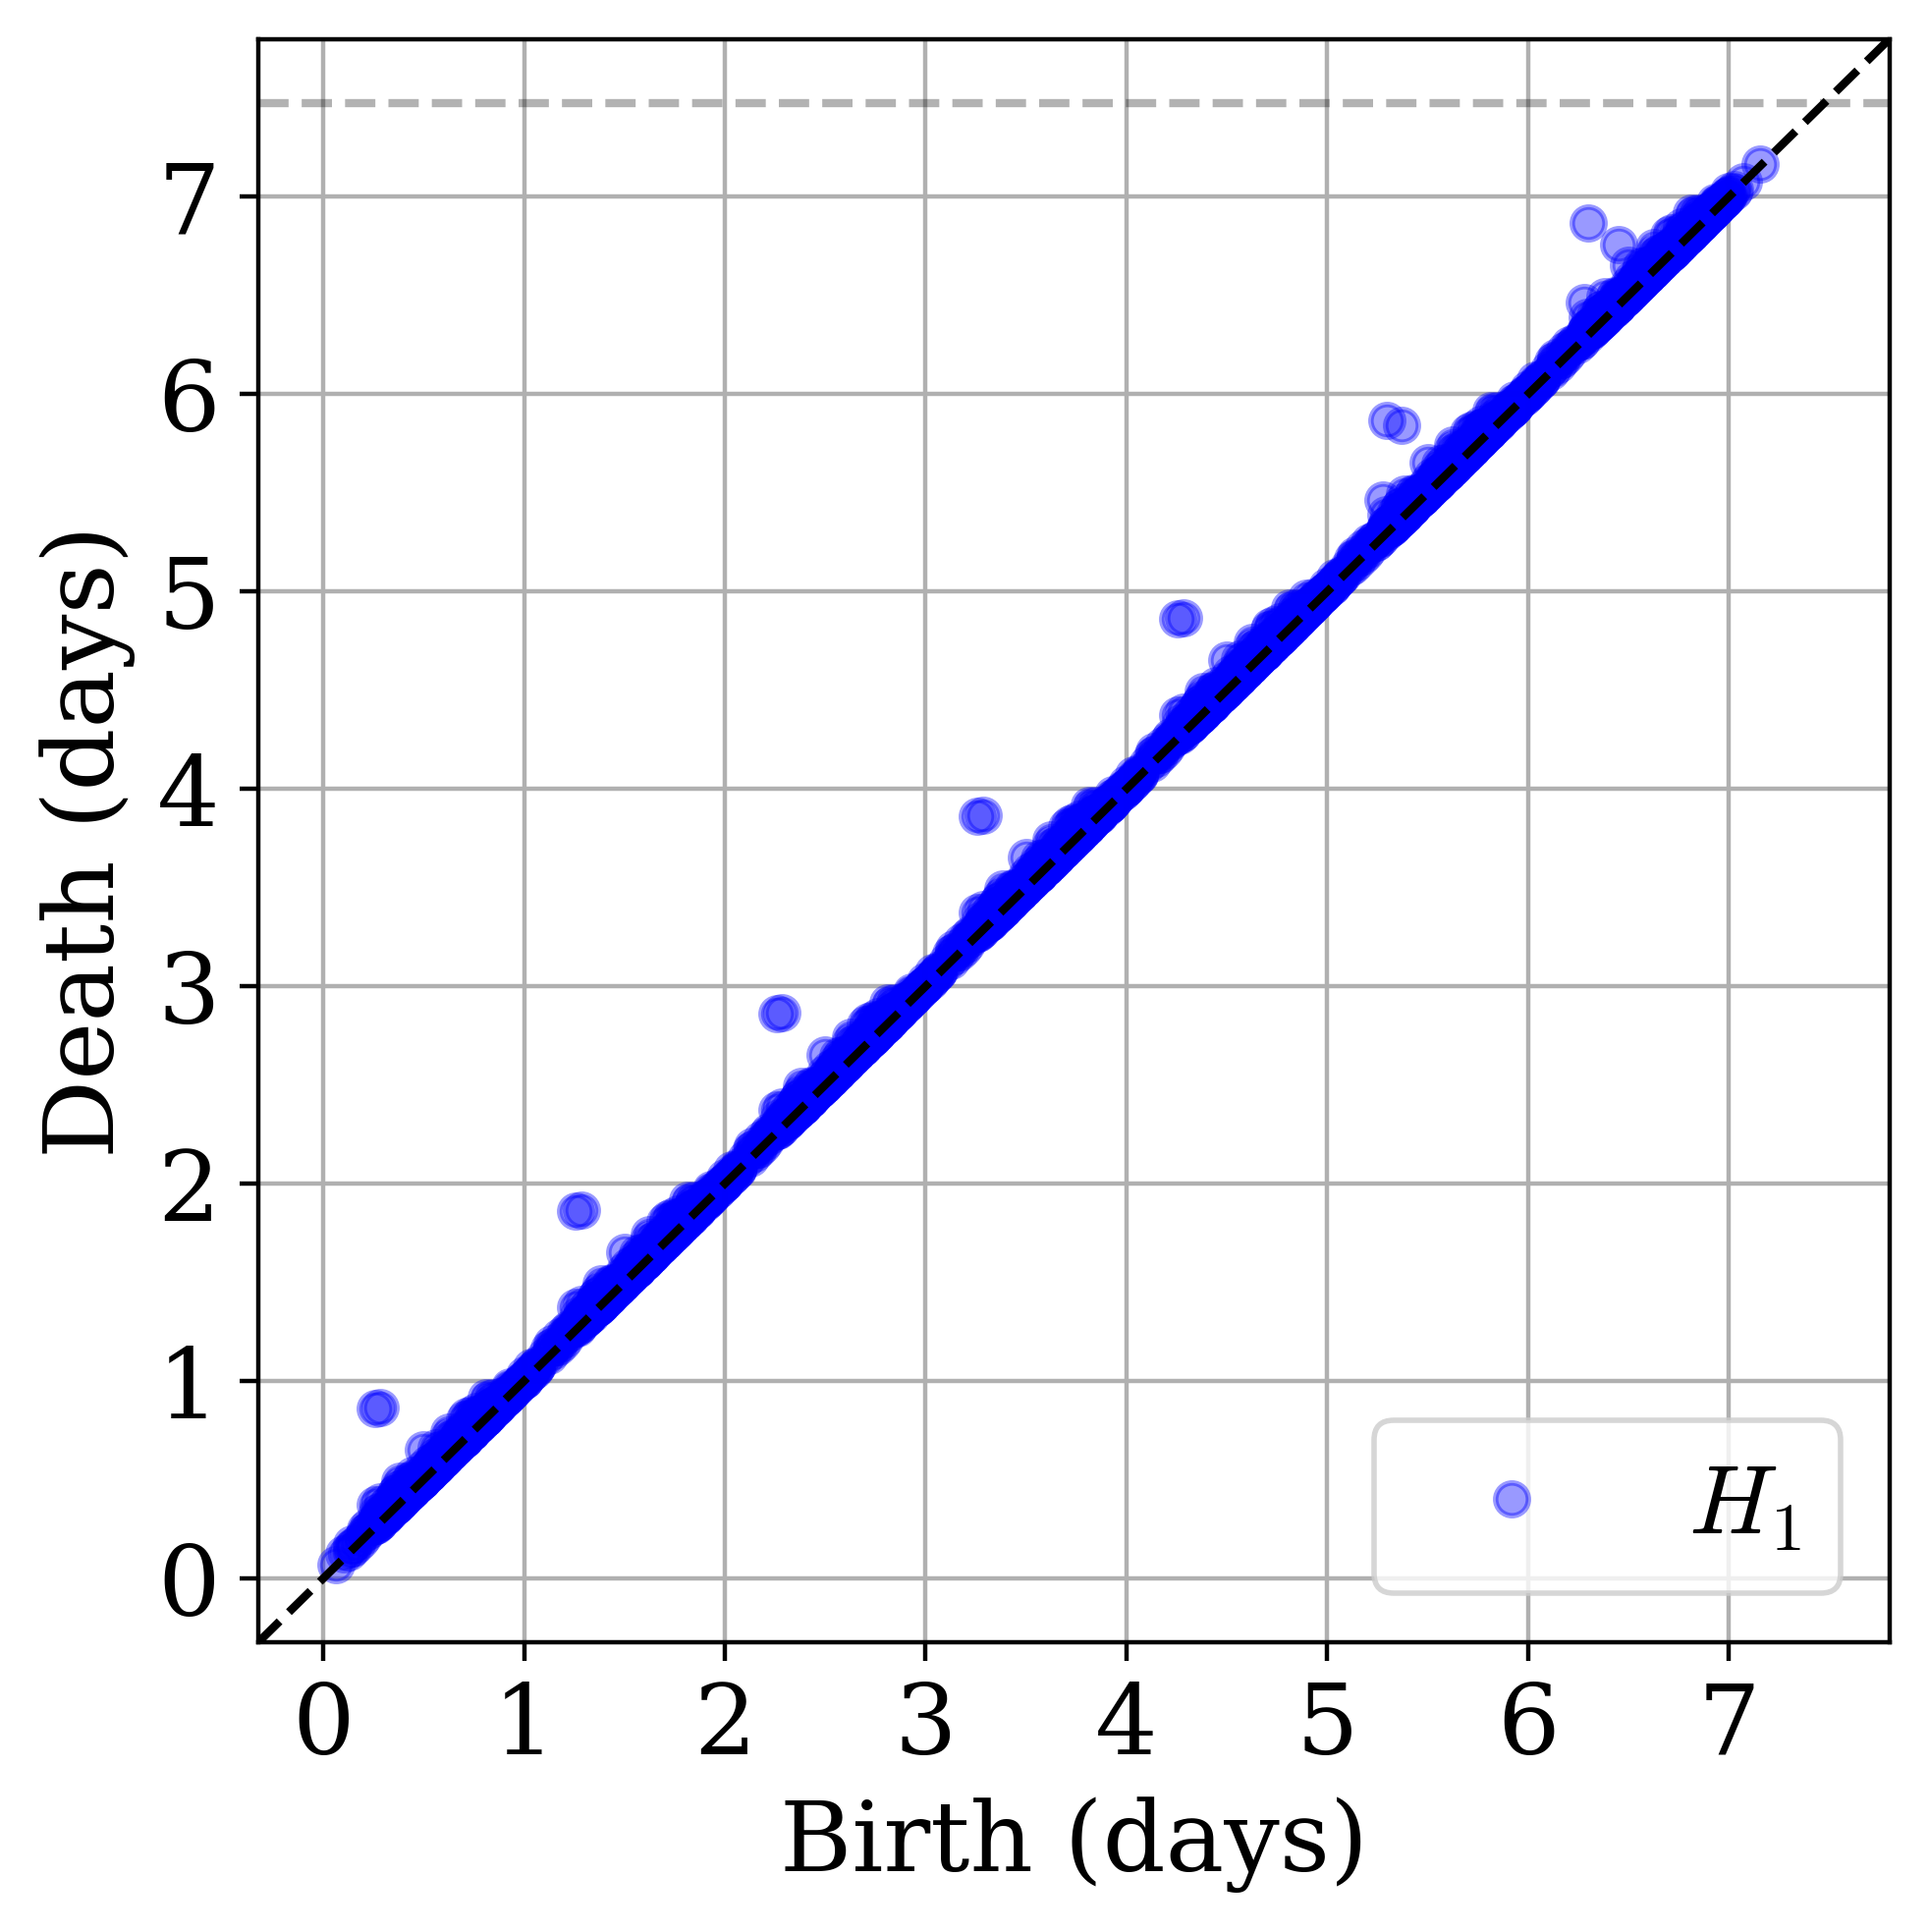
\includegraphics[width=\textwidth]{Figures/GB_coach_PD1_Rips1}
     \end{minipage}
     \hfill
     \begin{minipage}{0.31\textwidth}
         \centering
         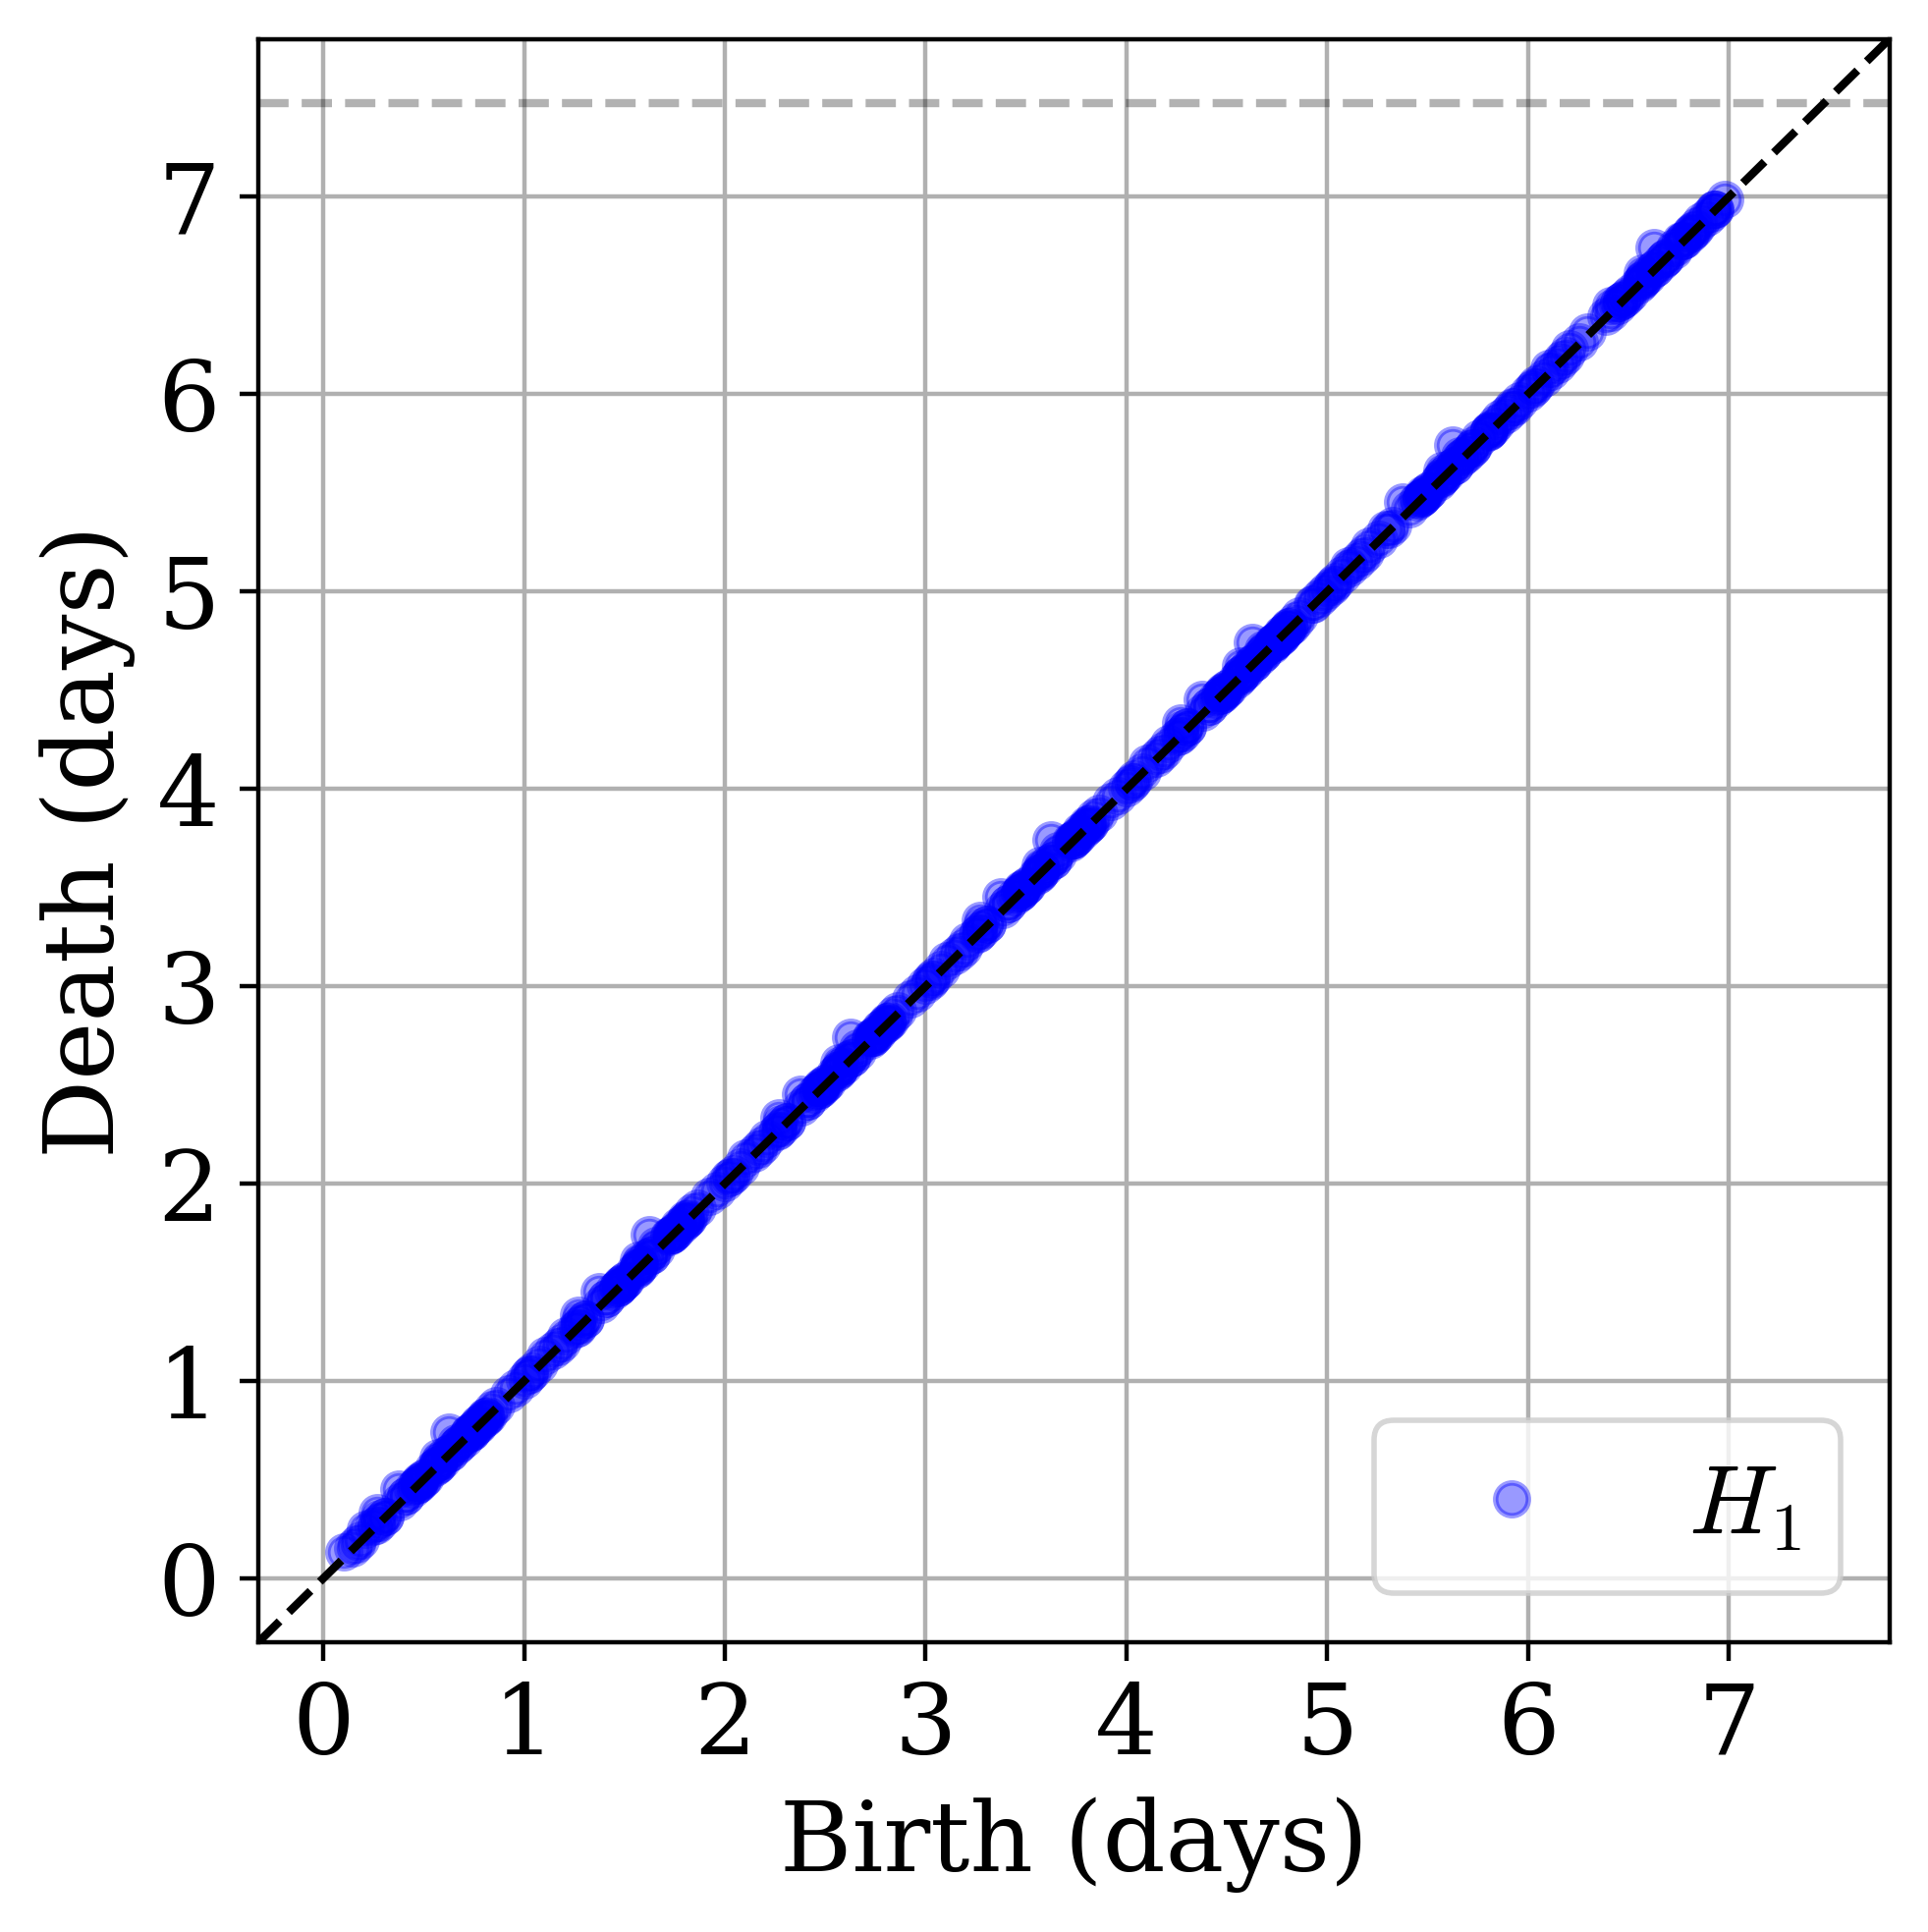
\includegraphics[width=\textwidth]{Figures/GB_coach_PD1_Rips2}
     \end{minipage}

     \begin{minipage}{0.31\textwidth}
         \centering
         (a) One-dimensional zigzag persistence using original graph.
     \end{minipage}
     \hfill
     \begin{minipage}{0.31\textwidth}
         \centering
         (b) One-dimensional zigzag persistence using VR complex with $r=1$.
     \end{minipage}
     \hfill
     \begin{minipage}{0.31\textwidth}
         \centering
         (c) One-dimensional zigzag persistence using VR complex with $r=2$.
     \end{minipage}
     %
     \caption{Zigzag persistence diagrams of the coach transportation network of Great Britain.}
     \label{fig:GB_coach_PD1s}
\end{figure}

\subsubsection{Coach}
\label{ssec:coach}
Now, we use the coach network data to illustrate using the VR complexes with different $r$ values. 
In Fig.~\ref{fig:GB_coach_PD1s}, 1-dimensional zigzag persistence diagrams are displayed. 
The leftmost diagram is computed using the graphs directly as input to the zigzag persistence without taking the VR complex.
The second and third were obtained using the graph and VR complexes with $r=1$ and $r=2$ respectively. 

Both diagrams (a) and (b) show periodic structure during the day which is to be expected as the number of buses running diminishes overnight. 
However, in diagram (b) we can clearly see a daily trend. 
While unfortunately difficult to see on the diagram, this is in fact points in the diagram overlaid, implying we have two loops of more than three edges that persist during the day. 
If the loops had length 3, they would be filled in by triangles when replacing the graph with the VR complex. 
This further implies that the noise seen in (a) is the existence of a great deal of triangles; not surprising in a highly connected local system like a bus network. 
But then, we can also compare persistence diagram Fig.~\ref{fig:GB_coach_PD1s}(b) to the analagous Fig.~\ref{fig:GB_rail_network_and_PDs}(c) from the rail network. 
The more locally connected nature of the bus system means that many of these small loops are not included when using the VR complex; however the rail system is more spread out, thus resulting in longer loops that are not filled in by a choice of $r=1$. 

Finally, we observe that in the persistence diagram of Fig.~\ref{fig:GB_coach_PD1s}(c), where there is very little of the periodic structure remaining. 
From this, we can assume that the many small loops seen in the $r=1$ diagram have been filled in by our choice of $r=2$, thus meaning that the loops are of length at most 6 (See the text surrounding Fig.6 of \cite{Myers2019} for a discussion of lifetime of loops by length in this setting).




%
%
%


\subsection{Temporal Ordinal Partition Network for Intermittency Detection} 
\label{ssec:TOPN_results}

In this section we apply the zigzag methods to study time series data encoded using complex networks; namely, the ordinal partition network.
Ordinal partition networks~\cite{McCullough2015} are a graph representation of time series data based on permutation transitions. 
As such, they encapsulate the state space structure of the underlying system. 
While we only use the ordinal partition network in this work, there are several other transitional complex networks from time-series data that a similar analysis could be done. These include $k$-nearest-neighbors~\cite{Khor2016}, epsilon-recurrence~\cite{Jacob2019}, and coarse-grained state-space networks~\cite{Small2009a,Small2013a}.
We begin by giving a brief introduction to the construction of the network from time series data, followed by the results of analysis using zigzag persistence.

\subsubsection{Temporal Ordinal Partition Network} 
\label{ssec:temp_OPN}
Given a time series $x = [x_0, x_1, x_2, \ldots, x_n]$ for a sequence of times $t = [t_0,\cdots, t_n]$, the ordinal partition network is formed by first generating a sequence of permutations  using a fixed permutation dimension $m$ and delay $\tau$. 
We generate a sequence of permutations by assigning each vector embedding 
\begin{equation}
v_i = [x_i, x_{i+\tau}, x_{i+2\tau}, \ldots, x_{i+(m-1)\tau}] = [v_i(0), v_i(1) \ldots, v_i(m-1)] 
\end{equation}
to one of the $m!$ possible permutations. 
We give an arbitrary ordering to the permutations for labeling purposes, and assign the permutation $\pi_j = [\pi_j(0), \ldots \pi_j(m-1)] \in \mathbb{Z}^{m}$ based on the ordinal pattern of $v_i$ such that 
$
v_i(\pi_j(0)) \leq v_i(\pi_j(1)) 
\leq 
\ldots \leq v_i(\pi_j(m-1))
$. 

Using the chronologically ordered sequence of permutations $\Pi$, we can form a graph $G(E,V)$ by setting the vertices $V$ as all permutations used and edges for transitions from $\pi_a$ to $\pi_b$ with $a, b \leq m!$ and $a \neq b$ (no self-loops). 
We will not add weight or directionality to the graph for this formation. 
However, we will track the index $i$ for the corresponding time $x_i$ when the edge is activated as the temporal data for the graph. 

\begin{figure}%
    \centering
    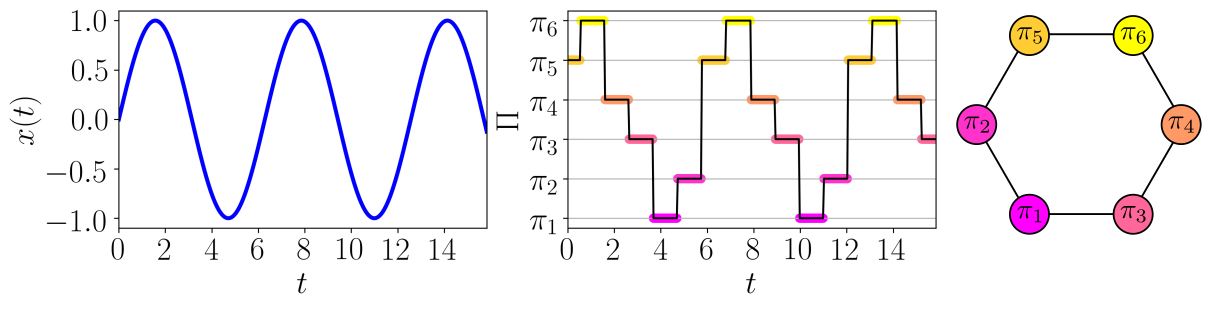
\includegraphics[width=0.82\textwidth]{Figures/simple_example_OPN_formation-FixedNotation.png}
    \caption{Example formation of an ordinal partition network for a sinusoidal signal $x(t) = \sin(t)$ with permutations of dimension $n=3$. The resulting permutation sequence $\Pi$ shows how these permutations transition, which is captured by the ordinal partition network on the right. 
    %
    }
    \label{fig:simple_example_OPN_formation}
\end{figure}

In Fig.~\ref{fig:simple_example_OPN_formation} we demonstrate the ordinal partition network formation procedure for a simple example signal as $x(t) = \sin(t)$, where $t \in [0,15]$ sampled at a rate of $f_s = 25$ Hz. 
Using the method of multi-scale permutation entropy we selected $\tau = 52$ and set $n=3$ for demonstrative purposes. The corresponding permutations to delay embedding vector $v_i$ is shown as a sequence $\Pi$ in the middle subfigure of Fig.~\ref{fig:simple_example_OPN_formation}. This sequence captures the periodic nature of the signal which is then summarized as the ordinal partition network on the right with each permutation as a vertex and edges added for permutation transitions in $\Pi$.
For more details and examples of the ordinal partition network, we direct the reader to~\cite{McCullough2015, Myers2019}. 

\subsubsection{Ordinal Partition Network Results}
Using a sliding window technique, we can represent ordinal partition networks as temporal graphs. 
However, instead of each edge having a set of intervals associated with it as in the example in Section~\ref{ssec:example}, they have time instances where the edge is active  based on when a transition between unique permutations occur. 
For example, the transition from $\pi_i$ to $\pi_{i+1}$ occurring at time $t_j$ would be active for the moment in time $t_j$. 
If the sliding window contains an edge's activation instance, we add that edge to the sliding window graph.

We will show how this procedure can be used to detect chaotic and periodic windows in a signal exhibiting intermittency (i.e., the irregular transitions from periodic to chaotic dynamics). 
The signal used here is the $z$
%
solution to the simulated Lorenz system defined as
\begin{equation}
\frac{dx}{dt}   = \sigma (y-x), \: \frac{dy}{dt}   = x (\rho -z) - y, \: \frac{dz}{dt}   = xy - \beta z
 \label{eq:lorenz}
\end{equation}
with system parameters $\sigma = 10$, $\beta = 8/3$, and $\rho = 166.18$ for a response with type 1 intermittency~\cite{Pomeau1980}.
We simulated the system with a sampling rate of 100 Hz for 500 seconds with only the last 70 seconds used.
%
To construct the ordinal partition network, we choose $m=6$ and $\tau$ using the multi-scale permutation entropy method as suggested in~\cite{Myers2020c}. 
We set the sliding windows for generating graph snapshots to have a width of $5\tau$ and $80\%$ overlap between adjacent windows. 

\begin{figure}%
    \centering
    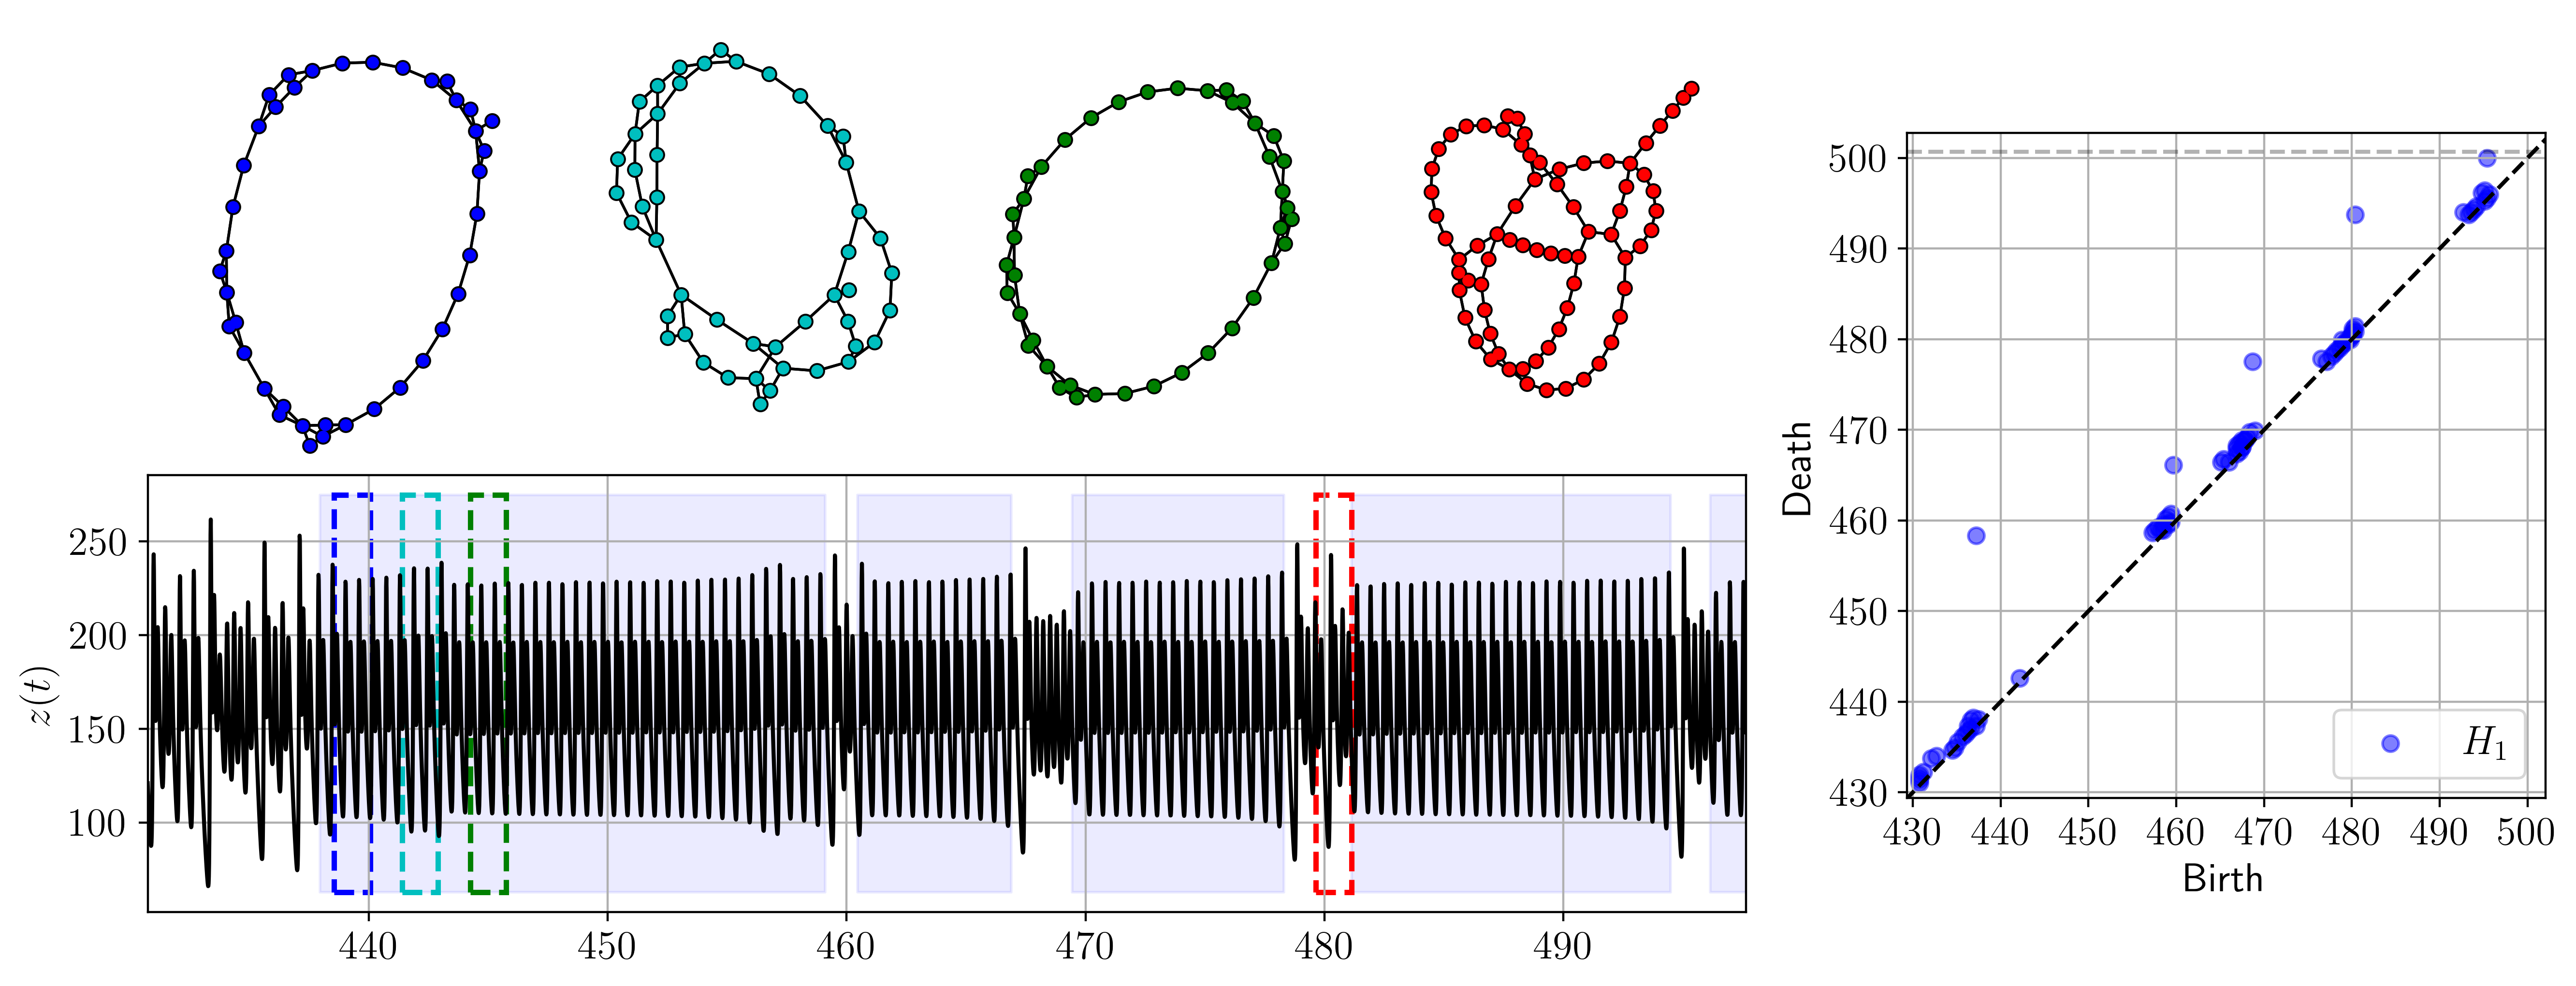
\includegraphics[width=0.99\textwidth]{Figures/intermittency_windows_and_PD1}
    \caption{One the left, the $z$ solution of the intermittent Lorenz system described in Eq.~\eqref{eq:lorenz} is shown, along with four different graphs obtained from the corresponding ordinal partition networks in the windows of matching color. On the right, the one-dimensional zigzag persistence diagram.}
    \label{fig:intermittency_windows_and_PD1}
\end{figure}
The resulting signal $z(t)$ from simulating the Lorenz system in Eq.~\eqref{eq:lorenz} is shown in Fig.~\ref{fig:intermittency_windows_and_PD1}, with four examples of ordinal partition networks generated at several window locations. 
These sample graph snapshots show that the structure of the ordinal partition network significantly changes depending on the dynamic state of the window's time-series segment. 
At right in the figure, we see the 1-dimensional zigzag diagram for the data. 
Of particular note is that there are several high persistence points in the diagram. 
Recalling that the coordinates of these points are associated to time of appearance of loops rather than size of the loops themselves, we have marked the regions of the times series associated to these points in blue at left. 
From visual inspection, it appears that these regions correspond to periodic behavior in the time series. 
The remaining chaotic windows characteristically have many low-lifetime persistence pairs seen close to the diagonal in the persistence diagram. 
This is in line with the results in~\cite{Myers2019} that showed ordinal partition networks from chaotic signals tend to have persistence diagrams with many features in $H_1$ when compared to their periodic counterpart.
The fact that this labeling is done with only the user's choice of threshold for what is considered a high-persistence point makes this a potentially exciting avenue for future work to understand how it can be used in the case of labeling intermittency in time series. 

Additionally, note in the persistence diagram in Fig.~\ref{fig:intermittency_windows_and_PD1} the point near the diagonal, at around second 442, representing a loop in the network that quickly disappears, as seen also in the first three ordinal partition networks shown at left of Fig.~\ref{fig:intermittency_windows_and_PD1}. This tells us that low-lifetime loops may show up in the middle of periodic regions while the main periodic trend is preserved, confirming that we can still trust the coordinates of high persistence points as the bounds of periodic regions.
Thus, in general, we can use the persistence diagram to identify periodic regions by looking for intervals where there are persistent loops over relatively long periods and very few (or no) other shorter-living loops, which is easily identified from the persistent points coordinates.
%

To compare with the standard tools from temporal network analysis, we show the connectivity and centrality measures of the graph snapshots in Fig.~\ref{fig:intermittency_mean_centrality_components_analysis}. 
The number of components $N_{cc}$ is constant due to the nature of the ordinal partition network, where the sequence of permutation transitions creates a chain of connected edges. 
As such, there is no structural information in the number of components. 
However, the size of the components does increase during the chaotic windows. This increase is due to, in general, more unique permutations and thus nodes used in a chaotic signal compared to periodic.
Of the centrality statistics, only the average closeness centrality shows an apparent increase during chaotic regions. 
The increase in centrality is most likely due to the chaotic regions causing a more highly connected graph as demonstrated in the chaotic window and corresponding network of Fig.~\ref{fig:intermittency_mean_centrality_components_analysis}.
While these statistics do provide some insight into the changing dynamics, they do not show how the higher-dimensional structure of the graph evolves through the sliding windows and graph snapshots, in contrast to zigzag persistence.

\begin{figure}%
    \centering
    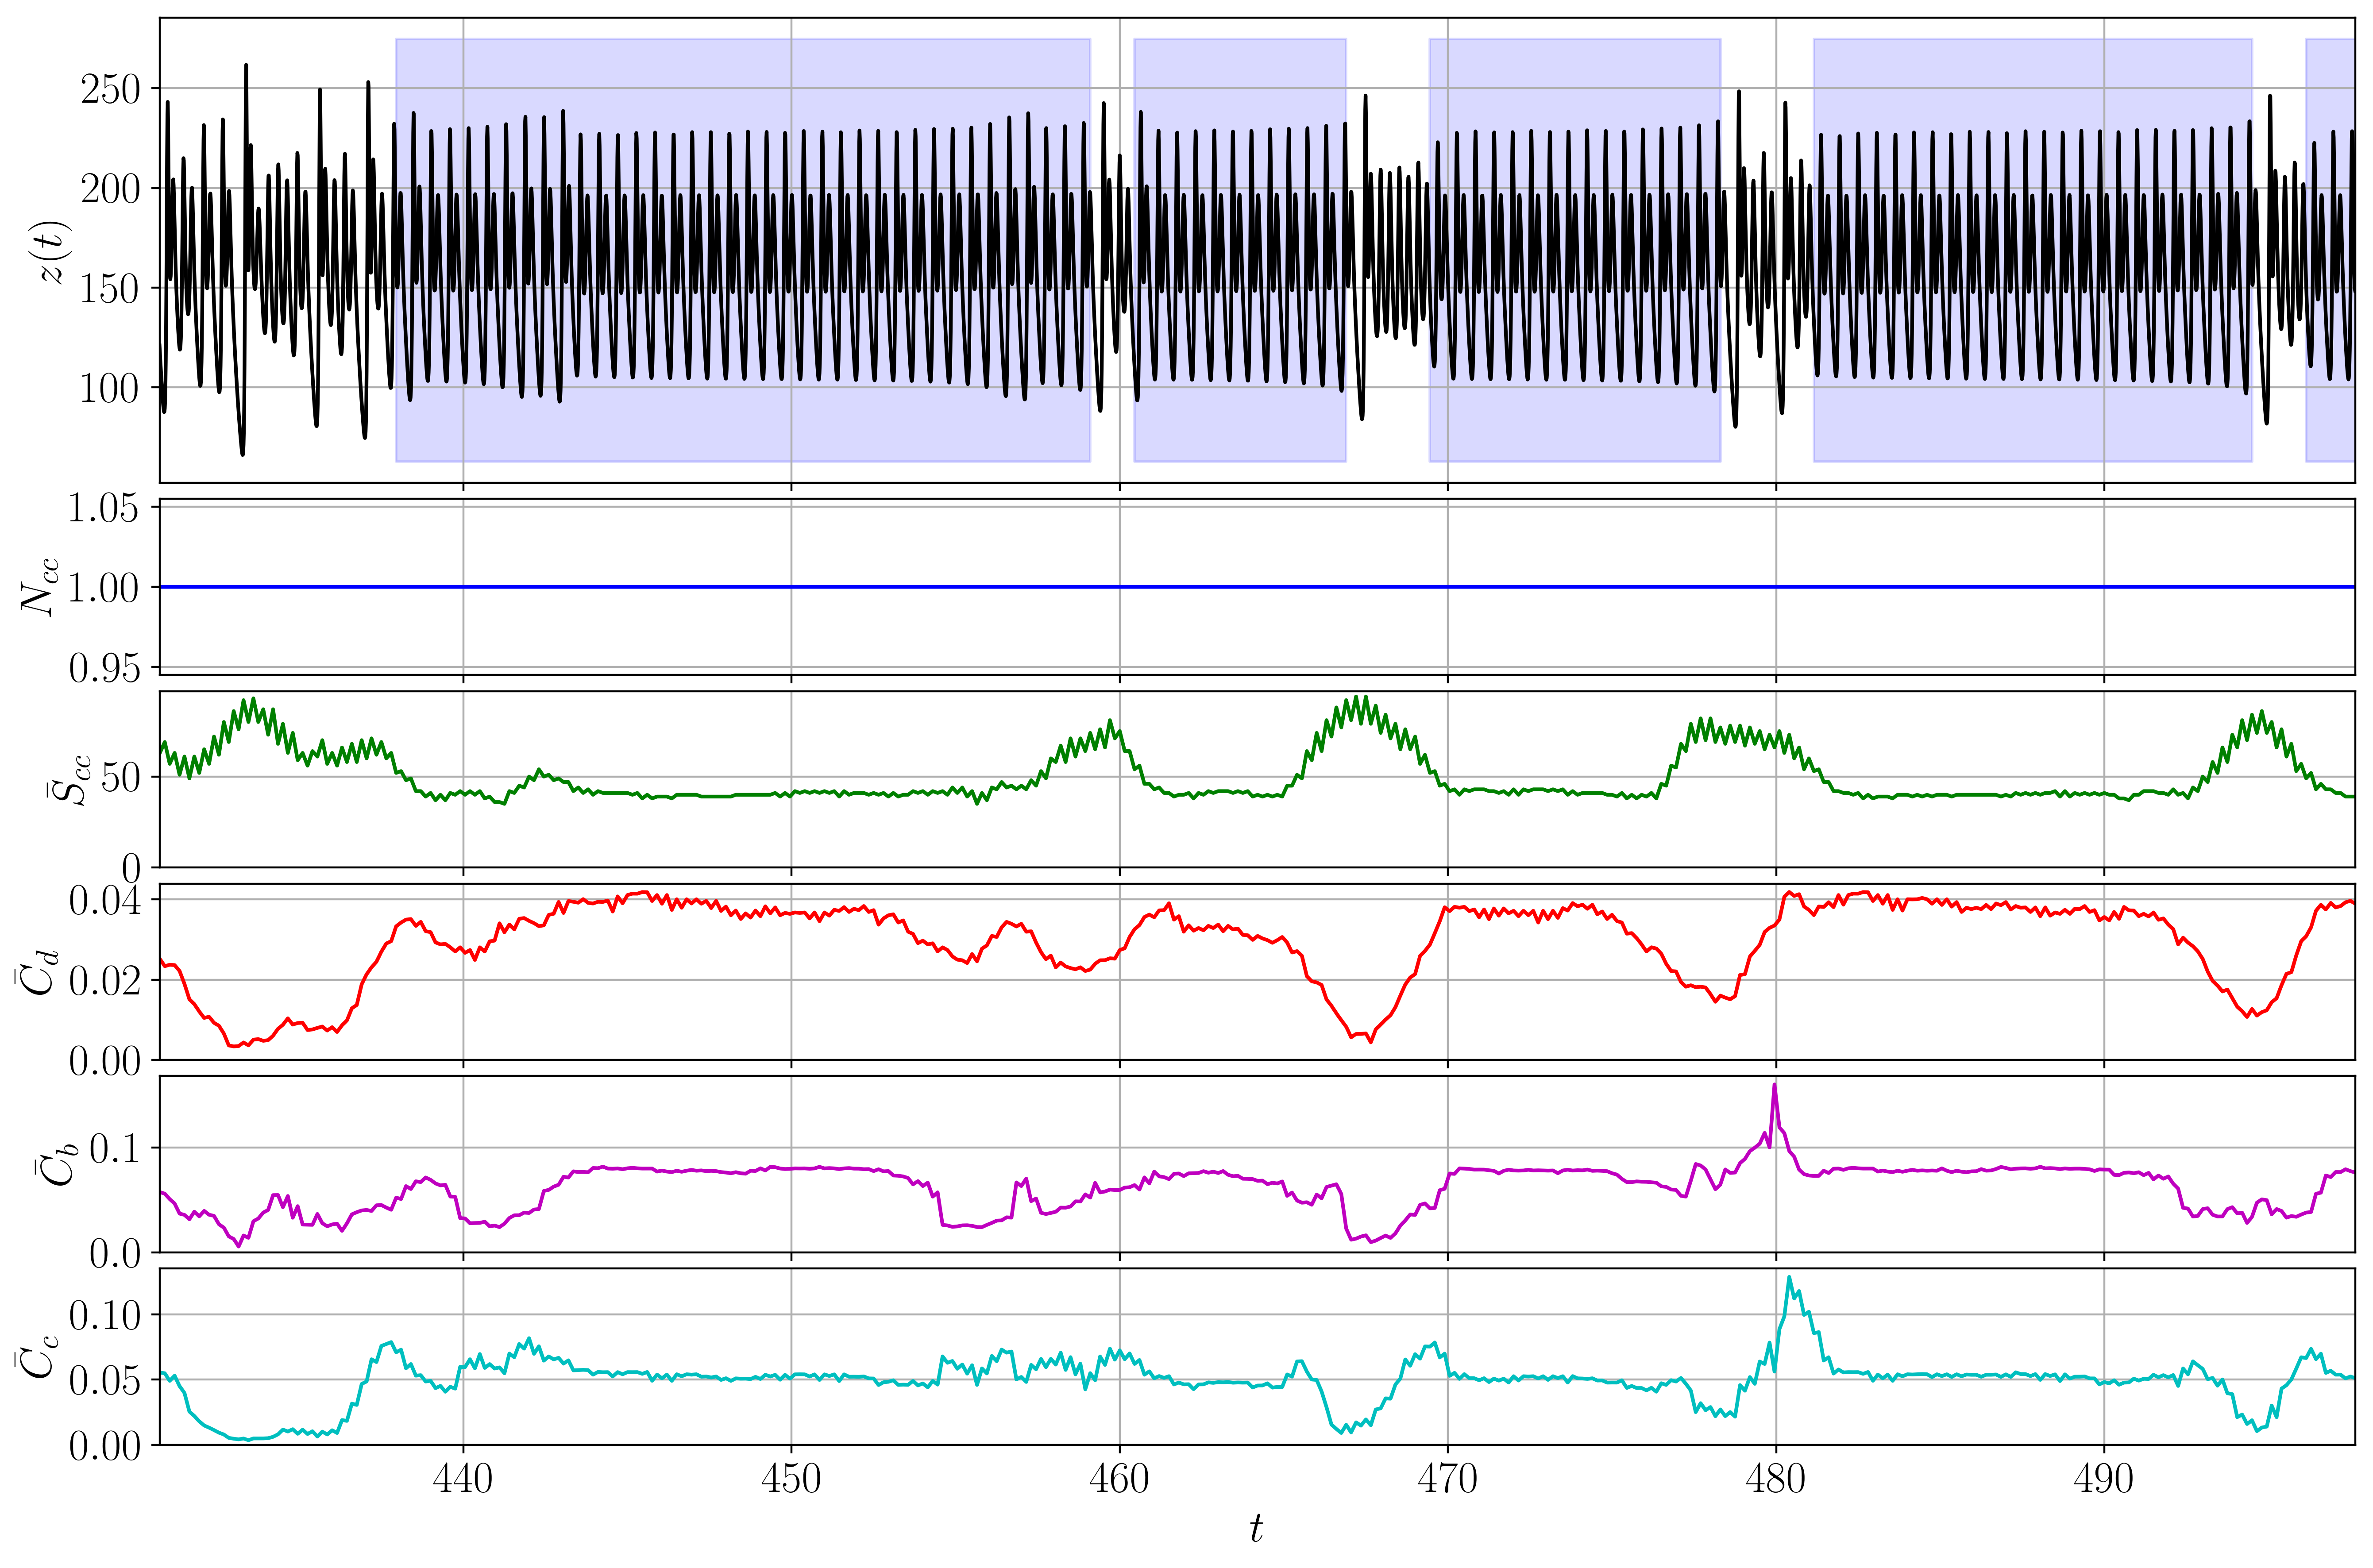
\includegraphics[width=0.99\textwidth]{Figures/intermittency_mean_centrality_components_analysis}
    \caption{Connectivity and centrality analysis on temporal ordinal partition network with periodic regions as labeled with the zigzag persistence points highlighted in blue.}
    \label{fig:intermittency_mean_centrality_components_analysis}
\end{figure}






